\documentclass{article}
\usepackage[pdftex]{graphicx}
\begin{document}
\title{Root isolation for one-variable polynomials}
\author{Yves Bertot, Assia Mahboubi, Fr\'ed\'erique Guilhot}

\maketitle

\section{introduction}
We want to describe an algorithm that isolates the roots of any
one-variable polynomial with rational coefficients.  This algorithms
constructs a finite list of intervals such that each interval contains
exactly one root of the polynomial and each root is in one of the
intervals.  Such an algorithm can be used as a basic bloc for other
algorithms, for instance to define algebraic numbers or as a component
of cylindrical algebraic decomposition, an algorithm known to decide
systems of inequations between polynomial formulas.

An operation that we will not cover in this paper is an operation
 to reduce the multiplicity of roots: this operation finds a new
polynomial that has the same roots, but where each root is simple.
This can easily be done by computing the greatest
common divisor between the polynomial and its derivative.  In the
following, we thus assume that our polynomial only has simple roots.

The approach we study is based on Bernstein coefficients.  These
coefficients give a discrete approximation of the behavior of a
polynomial in a given closed interval.  We rely on a sufficient
condition concerning these coefficients (let's call this condition
C1): if the Bernstein coefficients, taken in order, have only one
alternation, then the polynomial is guaranteed to have exactly one
root in the corresponding interval.

A first part of our work is to provide a mechanical proof of condition C1.

There are a collection of known transformation of polynomials, so that 
a given polynomial \(P\) has a root inside an interval \((l,r)\) if and
only a transformed polynomial \(P_1\) has a root inside the interval \((0,1)\).
Moreover,  there is a transformation so that \(P_1\) has a root inside
\((0,1)\) if and only if a transformed polynomial \(P_2\) has a root inside
\((0,+\infty)\).  Thus, a sufficient criterion for the existence of a
unique root between 0 and \(+\infty\) yields a sufficient criterion for
the existence of a unique root in a bounded interval \((l,r)\).
This is the essence of a the proof of condition C1.

Descartes' law of sign provides a sufficient criterion for the existence
of a root between 0 and \(+\infty\).  This law expresses a relation between
the number of roots of a polynomial between 0 and \(+\infty\) and the number
of sign changes in the coefficients of this polynomial.  The number of sign
changes is larger than the number of roots, moreover, the difference between
the two numbers is a multiple of 2.

For our development, we only use a simple special case of Descartes' law
of sign for the case where the coefficients of a polynomial
have only one sign change and express that there is a single simple root
between 0 (excluded) and positive infinity.  Expressing Descartes' law on
the coefficients of polynomial \(P_2\) yields directly a law expressed in terms
of sign changes for Bernstein's coefficients of \(P\) with respect to the
interval \((l,r)\).

Another part of our work is to describe dichotomy.  Knowing Bernstein
coefficients for a polynomial and a given interval, it is easy to
compute the Bernstein coefficients for the two half intervals, using
the algorithm known as "de Casteljau".  This increases the precision
at which the polynomials behavior is described, so that condition C1
is guaranteed to eventually hold in the dichotomy process.

Most of our proofs were made using only rational numbers as numeric
values.  Thus, we work with type of numbers where equality and
comparison are decidable and the process we described can effectively
be used in a decision procedure.

When considering only rational numbers, the existence of roots takes a
different meaning: if a polynomial has a single simple real root in an
interval, this root may not be rational.  However, we can use a
corresponding property on rational numbers: there exists a
sub-interval inside which the absolute value of the slope is bounded
below, and such that the values of the polynomial at the sub-interval
bounds have opposite signs.  In a similar vein, the intermediate value
theorem does not hold with rational numbers, but a corresponding
statement, expressed as an epsilon-delta property, does.  Our proof
development relies on this approach.

This result can then be used for several purposes.  First it opens the
door for a representation of algebraic numbers as equivalence classes
between pairs consisting of a polynomial with rational coefficients
and an interval.  Root isolation makes it possible to decide when two
such pairs describe the same algebraic number.  Second, it can be used
as a basic bloc for a decision procedure deciding logical formulas
with universal and existential quantification where atomic formulas
are comparisons between polynomial formulas.

Berstein polynomials and de Casteljau's algorithm are intensively used
in computer aided design.

\section{Describing simple roots in the rational setting}
Plan pour cette section
\begin{enumerate}
\item Roots of rational polynomials not necessarily polynomial
\item replace root as a number by a condition on evolution: decompose interval into three part: first part where the polynomial is proved to be strictly negative, second part where the polynomial goes from negative to positive with a slope that is strictly positive, third part where the polynomial is stricly positive
\item In case of Descartes law, impose the slope to be bounded below for all intervals but the first one
\item Using a new form of middle-value theorem: expressed only with rational numbers, applicable only for polynomials
\end{enumerate}
\section{A simple of form of Descartes' law of sign}
\subsection{Mathematical proof}
Let's first describe a simple graphical argument based on curves for polynomial functions between 0 and \(+\infty\), as shown in figure~\ref{graph-desc}.
\begin{figure}
\label{graph-desc}
\begin{center}
\includegraphics[width=0.5\textwidth]{alternated2.png}
\end{center}
{(a) non-negative coefficients, first one non-zero,\\
(b) non-negative coefficients, first one zero,\\
(c) first coefficient negative, all others non-negative,\\
(d) one sign change, first coefficient zero,\\
(e) one sign change, first coefficient negative}

\caption{Classes of polynomials with or without
sign change}
\end{figure}
To describe our proof, we assume that new polynomials are built from
existing ones by multiplying them by the polynomial \(X\) and adding a
constant; an operation that is known as ``Horner's scheme''.
Polynomials with one sign change and a positive principal coefficient
are obtained by starting with a positive constant, applying Horner's
scheme a certain number of times with non-negative constants, then
applying it a negative constant, and then applying it again a certain
number of times with non-positive constants.

Polynomials with only non-negative coefficients have curves which look
like the curves (3.1-a) or (3.1-b) depending on whether the first
coefficient is 0, adding a positive coefficient to a polynomial of the
form (a) or (b) yields a polynomial of the form (a), multiplying a
polynomial of the form (a) or (b) by the polynomial \(X\) yields a new
polynomial of the form (b).  Thus, Horner's scheme with non-negative
constants keeps polynomials in the (a-b) form.  Then, when applying
Horner's scheme with a negative coefficient (thus introducing a sign
change), the multiplication by \(X\) first builds a polynomial of the
(b) form, and adding a negative constant, one obtains a curve whose
shape is given by (c).  From then one, multiplying a polynomial of the
form (c), (d), or (e) by \(X\) yields a a polynomial of the (d) form; adding a
negative constant to a polynomial of the form (d) or (e) yields a
polynomial of the (e) form.  Polynomials of the form (d) or (e)
share the following characteristic: there exists a positive value
\(x\), so that the polynomial has a negative value between 0 and
\(x\), and the slope of the curve is strictly positive above
\(x\).  Because of the slope condition, we can also find a point where
the polynomial is positive.

Let us now give a more precise proof, outlining the concepts that are
used in the formal proof.

{\sf A lemma on slopes of products of functions: If two positive functions \(f\)
and \(g\) have slopes larger than \(k_f > 0\) and \(k_g > 0\) on the interval
\([a,b]\), then the slope
of the product \(fg\) is larger than \(k_fg(a) + f(a)k_g\).  \}

We first define an invariant that is used for polynomials with only
positive coefficients.  The important characteristics are the
following ones (grouped in our development under the name {\tt inv2}):
there exists a positive \(x\) such that \(x * P(x)\)
can be made arbirarily close to 0, the value of \(P(x)\) is positive,
the value of \(P\) in \([0,x]\) is below \(P(x)\), and the polynomial
is increasing above \(x\).  We then show that if any polynomial \(P\)
satisfies these important characteristics, and \(a\) is a non negative
number, then the polynomial \(a + X * P\) also satisfies them.

This is the step case in a proof by induction concerning polynomials
with all non-negative coefficients and at least one positive coefficient.

We can then address polynomials with exactly one alternation.  We want to
show that these polynomials have exactly one root.  We exhibit the three
intervals described in the previous section by giving two values \(x_1\) and \(x_2\) and \(k\) such that the polynomial is negative for every positive \(y\) smaller than \(x_1\), the polynomial is positive in \(x_2\), and the slope between
any two values above \(x_1\) is positive.
\begin{enumerate}
\item Consider a polynomial \(P = a_0 + a_1 x + a_n x^n\)
of degree \(n\), with two natural numbers \(i\), \(j\) such that
\(i < j\), \(a_i < 0\), \(0 < a_j\), and
\[\forall l, l < j \Rightarrow a_k \leq 0\]
\[\forall l, j \leq l \Rightarrow 0 \leq a_l\]
\item Prove that there is exactly one root between 0 and \(+\infty\)
\item Expressed in the following form: there exists \(x > 0\), \(k > 0\),
\(\forall y, 0 < y \leq x \Rightarrow P(y) < 0\) and
\(\forall y z, x \leq y < z \Rightarrow k (z - x) < P(z)-P(x) \).
\item The proof is done by two inductions:
\item First prove that every polynomial with only strictly positive coefficients
is strictly positive and increasing in \((0,+\infty)\)
\item Then prove by induction on \(j\)
\item Consider the truncated polynomial
\(P_t = a_1 + a_2 x + a_j x^{j-1} + a_n x^{n-1}\): we know that \(a_0 \leq 0\)
and there are two cases:
\begin{enumerate}
\item If \(P_t\) has no alternance, then \(a_0 < 0\) and the previous lemma
is satified for \(a_1 x + a_n x ^ n\) , this makes it possible to find
an \(x_1\) such that \(x_1 \times P(x_1) < - a_0\).  Thanks to the lemma
on slopes, the slope of the polynomial \(X \times P\) above \(x_1\) is larger
than \(P_t (x)\), this is enough to find a value \(x_2\) such that 
\(P(x_2)\) is positive.
\item If \(P_t\) has one alternance, then the induction hypothesis provides
a relevant \(x_{1t}\) and \(k_t\) for this polynomial.  We can consider the
value \(y = x_{1t} - a_0/{k_tx_{1t}}\).  This value is larger than \(x_{1t}\).
Thanks to the properties of \(k_t\) we know
that\(y * P_t(y) > k_t (y - x_{1t}) > - a0\) and thus, \(P(y) > 0\)
\item Using the middle-value theorem, we exhibit two new values \(z\) and \(x\),
 such that \(x_{1t} < z < x < y\), \(- k_t x_{1t} < P_t(z) < 0 < P_t(x) < a_0/y\)
\item Obviously, \(P\) is negative below \(x_{1t}\),
\item Thanks to the lemma at the beginning of this section, 
\(X * P_t\) has a slope larger than \(k * x_{1t} + P_t(z) > 0\) between
\(z\) and \(x\), so that \(P\) is negative in this interval,
\item Because \(P_t\) is increasing between \(x_{1t}\) and \(z\), \(P_t\) is
negative in
\item Because \(P_t\) is increasing between \(x_{1t}\) and \(x\), we can show
that \(P\) is negative between \(x_{1t}\) and \(x\)
\item  Thanks to the lemma at the beginning of this section,
the slope of \(P\) above \(x\) is larger than
\(k = P_t(x) + k_t x\).
\end{enumerate}
\end{enumerate}
\subsection{Formal description}
\begin{enumerate}
\item The functions that describe
\end{enumerate}
\end{document}
%%% Local Variables: 
%%% mode: latex
%%% TeX-master: t
%%% End: 
